\documentclass[preprint,proceedings]{rmaa}


%%%
%%% Define any personal macros here
%%% 

% These are some I use in typesetting example code
\newcommand{\bs}{\textbackslash}
\newcommand{\CS}[1]{\texttt{\textbackslash #1}}
% roman subscripts in math
\newcommand{\Sub}[1]{_\mathrm{#1}}
% a command to specify possible linebreak points in an email address 
\newcommand{\D}{\discretionary{}{}{}}

%%%
%%% Article preamble commands (title, authors, abstract, etc.) 
%%% None of these produce any output themselves, they just set things 
%%% up for \maketitle
%%%

% This is only used for making the header for the preprint version
\SetYear{2016}
\SetConfTitle{XV LARIM}

% Please use mixed case here, since this title gets propagated onto
% the web page, ADS entry, etc. 
  \title{The influence of environment on the HI mass functions in cosmological simulations}
  
 \author{Jesus D. Prada-Gonzalez\altaffilmark{1}, Michael G. Jones \altaffilmark{2}, J. E. Forero-Romero\altaffilmark{1} and Martha P. Haynes \altaffilmark{2}}

\altaffiltext{1}{Departamento de F\'isica, Universidad de los Andes,
    Cra 1 18A-10, Bloque Ip, Bogot\'{a}, Colombia.}
    
\altaffiltext{2}{Center for Radiophysics and Space Research,
  Space Sciences Building, Cornell University, Ithaca, NY
  14853, USA.}



  % List of authors used to construct table of contents
  \listofauthors{Jesus Prada, Michael G. Jones, J. E. Forero-Romero and Martha P. Haynes}
  % Each author in Surname, Initials format, used in generating Author
  % Index entries.
  \indexauthor{Prada-Gonzalez, J. D.}
  \indexauthor{Jones, M. G.}
  \indexauthor{Forero-Romero, J. E.}
  \indexauthor{Haynes, M. P.}


% No \abstract or \resumen for poster papers

% Keywords must be from the standard list and in alphabetical order. 
\addkeyword{HI mass funcions}
\addkeyword{Environment}
\addkeyword{Schechter functions}
\addkeyword{Nearest neighbour}
\addkeyword{Cosmic web}


%%%
%%% Beginning of document proper
%%%
\begin{document}
% Typeset article header
\maketitle 
%%%Resumen en Español%%%
\boldabstract{En este proyecto verificamos en la simulaci\'on Illustris el efecto del entorno sobre las funciones de masa de galaxias. Descubrimos, con dos definiciones de entorno de naturaleza distinta, que este afecta claramete el parámetro knee-mass de las funciones de Schechter asociadas a las funciones de masa mientras que su efecto sobre el parámetro faint-end slope es difuso. Esto concuerda con lo encontrado por Jones et al.}

%%%Abstract%%%

\boldabstract{We study the effect of environment on mass functions of galaxies from Illustris simulation. We discovered, with the use of two definitions of environment of different nature, that the environment clearly affects the Knee-mass parameter of the Schechter functions associated with the mass functions, while the effect on faint-end slope parameter is diffuse. This is in accordance to the study by Jones et al.}\\

We obtained the Schechter functions of baryonic mass corresponding to groups of galaxies classified by two different criteria for the definition of environment. The first definition is a computational adaptation of the fourth nearest neighbour method used by Jones et al. in their observational study. We classified galaxies in four quartiles according to this environment definition and obtained the mass and Schechter functions for each one. In \ref{fig1} the environments are shown in crescent order of density from top to bottom.

\begin{figure}[h!]
\centering
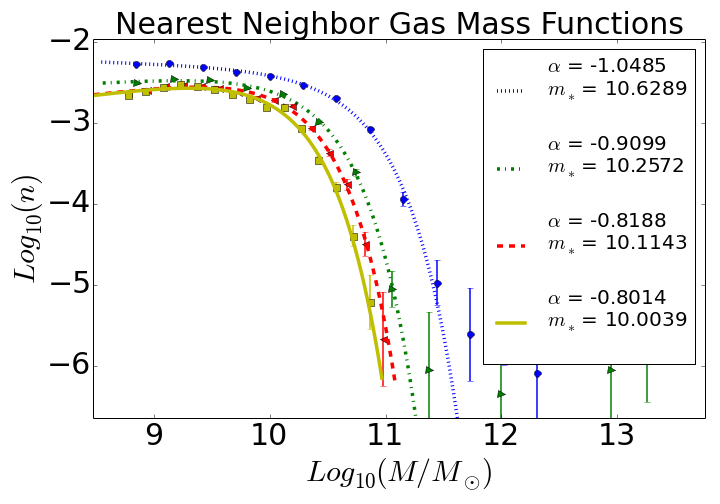
\includegraphics[width=0.5\textwidth]{environment1}
\label{fig1}
\caption{4th nearest neighbour environmental dependence of mass functions}
\centering
\end{figure}

The second definition of environment is of computational nature which was proposed by Forero et al. It takes the density field of the simulation to calculate the Hessian of the gravitational potential and according to this, it classifies the morphology of potential wells in four environments: voids, filaments, sheets and clusters. The result of the Schechter functions for these environments are shown in \ref{fig2}, where environments are shown in crescent order of density from top to bottom.

\begin{figure}[h!]
\centering
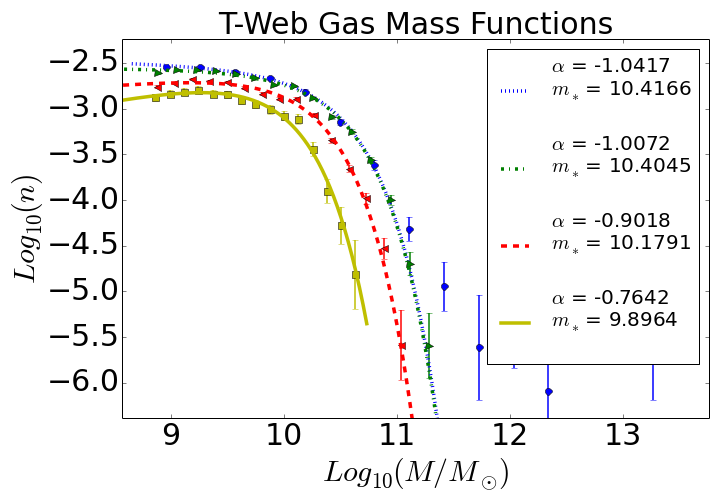
\includegraphics[width=0.5\textwidth]{environment2}
\label{fig2}
\caption{Morphological environmental dependence of mass functions}

\centering
\end{figure}

 With some analysis of errors of the Schechter fits it is demonstrated that the effect of environment is clear for the knee-mass, while for the faint-end slope, the variation is so subtle to make conclusions with this methods. This is in accordance with the study by Jones et al. \\
 
\begin{thebibliography}
\bibitem{Jones}M. G. Jones, E. Papastergis, M. P. Haynes, and R. Giovanelli. Environmental dependence of the H I mass function in the ALFALFA 70\% catalogue. MNRAS, 457:4393–4405, April 2016.
\bibitem{Forero}J. E. Forero-Romero, Y. Hoffman, S. Gottl ̈ober, A. Klypin, and G. Yepes. A dynamical classification of the cosmic web. MNRAS, 396:1815–1824, July 2009.

  
\end{thebibliography}

\end{document}
